\documentclass[10pt,twocolumn,a4paper]{article}

\usepackage[a4paper,margin=16mm,columnsep=7mm]{geometry}
\usepackage{mathptmx}
\usepackage{amsmath,amssymb,amsthm,mathtools}
\usepackage{graphicx}
\usepackage{booktabs}
\usepackage{tabularx}
\usepackage{caption}
\usepackage{subcaption}
\usepackage{xcolor}
\usepackage{microtype}
\usepackage{cite}
\usepackage[hyphens]{url}
\usepackage{hyperref}

\definecolor{primary}{RGB}{24,78,119}
\hypersetup{
    colorlinks=true,
    linkcolor=primary,
    citecolor=primary,
    urlcolor=primary,
    pdftitle={Degree Heterogeneity, Eigenvector Localization, and Regime Interactions in Ordinary and Normalized Spectral Graph Clustering},
    pdfauthor={Lakshya (Department of Computer Science and Engineering, IIT Delhi)}
}

\setlength{\parskip}{2.8pt plus 1pt minus 1pt}
\captionsetup{font=small,labelfont=bf}

\title{\vspace{-8mm}\textbf{Degree Heterogeneity, Eigenvector Localization, and Regime Interactions in Ordinary and Normalized Spectral Graph Clustering}}

\author{
  \textbf{Lakshya}\\
  Department of Computer Science and Engineering, Indian Institute of Technology Delhi\\
  Repository: \href{https://github.com/lakshya07iitd-ai/spectral-graph-clustering}{\texttt{github.com/lakshya07iitd-ai/spectral-graph-clustering}}
}
\date{November 2026}

\begin{document}
\sloppy

\maketitle

\begin{abstract}
Spectral graph clustering partitions networks using low-frequency eigenvectors of graph Laplacian operators, yet practitioners face a fundamental choice between the ordinary combinatorial Laplacian $L = D - A$ and the symmetric normalized Laplacian $L_{\mathrm{sym}} = D^{-1/2} L D^{-1/2}$. While asymptotic theory demonstrates that $L_{\mathrm{sym}}$ converges to a well-behaved compact integral operator under broad degree distributions whereas $L$ possesses a continuous multiplication spectrum spanning $[d_{\min}, d_{\max}]$, empirical benchmarks on finite graphs often confound node-level degree dispersion with community-size skew and shifted inter-community edge mixing. This paper presents a controlled experimental investigation of ordinary and normalized spectral clustering implemented from scratch in Python and NumPy. First, we show mathematically that naive degree-corrected stochastic block models (DC-SBMs) reduce expected within-community edge density as degree variance increases due to self-loop exclusion and hub-pair probability clipping. We resolve this confound by introducing a Separation-Calibrated DC-SBM that enforces exact within-community propensity normalization and bisection-calibrated edge expectations ($\mathbb{E}[m_{\mathrm{in}}] = 87.75$, $\mathbb{E}[m_{\mathrm{out}}] = 24.00$ on $N=30, K=3$ graphs). Second, across 90 matched trials at baseline separation ($p_{\mathrm{in}}=0.65, p_{\mathrm{out}}=0.08$), paired Adjusted Rand Index (ARI) gain $\Delta\mathrm{ARI} = \mathrm{ARI}_{\mathrm{norm}} - \mathrm{ARI}_{\mathrm{ord}}$ rises monotonically from $+0.0220$ ($p = 0.1718$, non-significant) under balanced degrees to $+0.0694$ ($p = 0.0307$) under moderate degree imbalance and $+0.0927$ ($p = 0.0089$) under high degree imbalance. Third, a two-way regime investigation across 450 graph instances reveals a strong interaction between degree heterogeneity ($\gamma$) and community mixing ($p_{\mathrm{out}}$): when communities are strongly separated ($p_{\mathrm{out}}=0.02$), both operators achieve $\mathrm{ARI} = 1.0000$, whereas under elevated mixing ($p_{\mathrm{out}}=0.22$) and high degree heterogeneity ($\gamma=0.85$), $\Delta\mathrm{ARI}$ reaches $+0.5509$ ($95\%$ CI $[+0.462, +0.640]$, Wilcoxon $p = 1.73\times 10^{-6}$). Mechanistic spectral diagnostics demonstrate that ordinary clustering failure is driven by peripheral eigenvector localization whenever the $k$-th Laplacian eigenvalue approaches the minimum vertex degree ($\lambda_3(L)/d_{\min} \to 1$), inflating the Inverse Participation Ratio ($\mathrm{IPR}(L)$ correlates with $\mathrm{ARI}_{\mathrm{ord}}$ at $r = -0.7494$). Finally, we identify the sparse hub-periphery regime ($p_{\mathrm{in}}=0.32, \bar{d}_{\min}=0.17$) where standard $L_{\mathrm{sym}}$ itself degrades to $\mathrm{ARI}=0.2134$ due to disconnected and pendant vertices, and verify that degree-regularized spectral clustering ($L_\tau$) restores accuracy to $\mathrm{ARI}=0.7357$.
\end{abstract}

\noindent\textbf{Keywords:} Spectral Graph Clustering, Graph Laplacian, Normalized Cut, Degree-Corrected Stochastic Block Model, Eigenvector Localization, Eigengap, Degree Regularization.

\section{Introduction}
Community detection in undirected networks is a foundational problem in machine learning, network science, and combinatorial optimization \cite{fortunato2010community,shi2000normalized}. Given an undirected graph $G = (V, E)$ with non-negative adjacency matrix $A \in \mathbb{R}_{\ge 0}^{n \times n}$, spectral clustering embeds vertices into $\mathbb{R}^k$ using the bottom $k$ eigenvectors of a graph Laplacian matrix and partitions the resulting embedding via $k$-means clustering \cite{ng2001spectral,vonluxburg2007tutorial}. Because spectral relaxations convert NP-hard discrete cut objectives into tractable symmetric eigenvalue problems \cite{fiedler1973algebraic,shi2000normalized}, they provide both mathematical transparency and strong empirical performance.

Despite identical computational complexity, two distinct Laplacian operators dominate the literature: the ordinary (unnormalized) Laplacian $L = D - A$, which relaxes RatioCut, and the symmetric normalized Laplacian $L_{\mathrm{sym}} = D^{-1/2} L D^{-1/2}$, which relaxes Normalized Cut (Ncut) \cite{shi2000normalized,vonluxburg2007tutorial}. On nearly regular graphs where all vertices share similar degrees, $D \approx \bar{d} I$ and the eigenvectors of $L$ and $L_{\mathrm{sym}}$ span nearly identical subspaces. Real-world networks, however, exhibit pronounced degree heterogeneity, combining high-degree hub vertices with low-degree peripheral vertices inside the same community \cite{karrer2011stochastic}.

\section{Research Motivation}
While theoretical analyses establish that unnormalized spectral clustering can fail asymptotically when the minimum degree $d_{\min}$ overlaps the nontrivial community eigenvalues of $L$ \cite{vonluxburg2008consistency}, finite-sample empirical studies frequently suffer from three methodological weaknesses:
\begin{enumerate}\setlength{\itemsep}{1pt}\setlength{\parskip}{0pt}
    \item \textbf{Confounded Graph Generation:} When synthetic graphs are generated via naive Degree-Corrected Stochastic Block Models (DC-SBMs) \cite{karrer2011stochastic}, increasing vertex propensity variance simultaneously alters within-community edge counts and community volume balance, confounding degree heterogeneity with community separation.
    \item \textbf{Confounded Algorithmic Choices:} Standard implementations of normalized spectral clustering apply Ng--Jordan--Weiss (NJW) spherical row normalization \cite{ng2001spectral}, leaving unclear whether empirical gains stem from the normalized operator $L_{\mathrm{sym}}$ or from post-eigenvector row normalization.
    \item \textbf{Single-Regime Overgeneralization:} Reporting a single benchmark setting obscures the boundary conditions where $L$ performs comparably to $L_{\mathrm{sym}}$ as well as the sparse regime where $L_{\mathrm{sym}}$ itself breaks down \cite{qin2013regularized}.
\end{enumerate}
This study addresses all three issues through a rigorously controlled empirical investigation built atop a verified from-scratch spectral graph library.

\section{Research Questions and Hypotheses}
Our primary research question asks: \emph{How does within-community degree heterogeneity affect the relative community recovery accuracy of ordinary ($L$) and symmetric normalized ($L_{\mathrm{sym}}$) spectral clustering when community separation and expected edge densities are held strictly constant, and how does this relationship vary across network mixing and sparsity regimes?}

We formulate and test three falsifiable hypotheses:
\begin{itemize}\setlength{\itemsep}{1pt}\setlength{\parskip}{0pt}
    \item \textbf{Hypothesis H1 (Monotonic Divergence at Fixed Separation):} At a fixed intermediate community separation where both methods succeed under homogeneous degrees, increasing within-community degree dispersion (measured by the degree coefficient of variation $\mathrm{CV}_d$) degrades ordinary spectral clustering while leaving normalized spectral clustering stable, yielding a positive and increasing paired accuracy gap $\Delta\mathrm{ARI} = \mathrm{ARI}_{\mathrm{norm}} - \mathrm{ARI}_{\mathrm{ord}}$.
    \item \textbf{Hypothesis H2 (Regime Interaction and Non-Uniformity):} The advantage of $L_{\mathrm{sym}}$ over $L$ is not uniform across graph structures; it vanishes when inter-community mixing is sufficiently low ($\lambda_k(L) \ll d_{\min}$) and amplifies super-additively as inter-community mixing pushes $\lambda_k(L)$ toward $d_{\min}$.
    \item \textbf{Hypothesis H3 (Peripheral Localization vs.\ Sparse Breakdown):} Ordinary clustering failures under degree heterogeneity are driven by eigenvector localization onto low-degree peripheral vertices rather than hub dominance; conversely, in sparse hub-periphery graphs where $d_{\min} \to 0$, standard $L_{\mathrm{sym}}$ loses its advantage unless stabilized by degree regularization ($L_\tau$).
\end{itemize}

\section{Relevant Literature Review}
Spectral graph partitioning originated with Fiedler's analysis of the second smallest eigenvalue $\lambda_2(L)$ (algebraic connectivity) and its eigenvector for two-way graph bisection \cite{fiedler1973algebraic}. Shi and Malik \cite{shi2000normalized} demonstrated that minimizing raw cut or RatioCut often isolates single low-degree vertices and introduced the Normalized Cut criterion, showing that its continuous relaxation is solved by the generalized eigenvalue problem $L x = \lambda D x$, equivalent to the standard eigenvalue problem for $L_{\mathrm{sym}} = D^{-1/2} L D^{-1/2}$. Ng, Jordan, and Weiss \cite{ng2001spectral} extended symmetric normalized spectral clustering to $k$ communities by projecting the bottom $k$ eigenvectors of $L_{\mathrm{sym}}$ onto the unit sphere via row normalization prior to $k$-means clustering.

From a statistical perspective, von Luxburg, Belkin, and Bousquet \cite{vonluxburg2008consistency} proved a fundamental dichotomy: as sample size $n \to \infty$, $L_{\mathrm{sym}} = I - D^{-1/2}AD^{-1/2}$ is a compact perturbation of the identity whose isolated bottom eigenvalues converge consistently, whereas $\frac{1}{n}L$ converges to a multiplication operator whose continuous essential spectrum spans the range of the degree function. Consequently, whenever a nontrivial cluster eigenvalue lies inside $[d_{\min}, d_{\max}]$, the corresponding sample eigenvector localizes around a single low-degree vertex \cite{vonluxburg2007tutorial,vonluxburg2008consistency}.

To model real-world networks with broad degree distributions, Karrer and Newman \cite{karrer2011stochastic} proposed the Degree-Corrected Stochastic Block Model (DC-SBM). Rohe, Chatterjee, and Yu \cite{rohe2011spectral} proved high-dimensional consistency of $L_{\mathrm{sym}}$ under dense SBMs using Davis--Kahan subspace perturbation bounds \cite{yu2015useful}. Subsequently, Chaudhuri et al.\ and Qin and Rohe \cite{qin2013regularized} showed that under sparse DC-SBMs with very low-degree vertices, $L_{\mathrm{sym}}$ suffers from high variance on pendant and isolated vertices, motivating the regularized Laplacian $L_\tau = I - D_\tau^{-1/2} A D_\tau^{-1/2}$ with $D_\tau = D + \tau I$.

\emph{Distinction of Our Contribution:} The theoretical properties of $L$, $L_{\mathrm{sym}}$, and $L_\tau$ are established in the literature \cite{vonluxburg2008consistency,karrer2011stochastic,qin2013regularized}. Our contribution is a rigorous finite-sample experimental methodology and mechanistic verification: we derive and correct the finite-graph self-loop and clipping confounds in DC-SBM benchmarking, decouple operator normalization from spherical row normalization via explicit ablations, and quantify how the spectral threshold ratio $\lambda_3(L)/d_{\min}$ and Inverse Participation Ratio ($\mathrm{IPR}$) govern finite-graph failure modes.

\section{Mathematical Background}
Let $G = (V, E)$ be an undirected simple graph on $n = |V|$ vertices with symmetric adjacency matrix $A \in \{0,1\}^{n \times n}$ ($A_{ii} = 0$). The vertex degrees are $d_i = \sum_{j=1}^n A_{ij}$, forming $D = \mathrm{diag}(d_1, \dots, d_n)$. The ordinary graph Laplacian is:
\begin{equation}
    L = D - A.
\end{equation}
For any vector $x \in \mathbb{R}^n$, $L$ satisfies the edge-based quadratic form identity:
\begin{equation}
    x^T L x = \frac{1}{2} \sum_{i=1}^n \sum_{j=1}^n A_{ij} (x_i - x_j)^2 \ge 0.
    \label{eq:quadform}
\end{equation}
Thus $L$ is symmetric positive semi-definite with eigenvalues $0 = \lambda_1(L) \le \lambda_2(L) \le \dots \le \lambda_n(L)$, and the multiplicity of the zero eigenvalue equals the number of connected components of $G$ \cite{vonluxburg2007tutorial}.

Defining the safe inverse square-root degree matrix $D^{-1/2} = \mathrm{diag}(d_1^{-1/2}, \dots, d_n^{-1/2})$ with $d_i^{-1/2} \coloneqq 0$ whenever $d_i = 0$, the symmetric normalized Laplacian is:
\begin{equation}
    L_{\mathrm{sym}} = D^{-1/2} L D^{-1/2} = I_{\mathrm{pos}} - D^{-1/2} A D^{-1/2},
\end{equation}
with eigenvalues $0 = \lambda_1(L_{\mathrm{sym}}) \le \lambda_2(L_{\mathrm{sym}}) \le \dots \le \lambda_n(L_{\mathrm{sym}}) \le 2$. Its quadratic form normalizes each vertex value by $\sqrt{d_i}$:
\begin{equation}
    x^T L_{\mathrm{sym}} x = \frac{1}{2} \sum_{i=1}^n \sum_{j=1}^n A_{ij} \left(\frac{x_i}{\sqrt{d_i}} - \frac{x_j}{\sqrt{d_j}}\right)^2.
\end{equation}
For a two-way partition $(S, \bar{S})$, with $\mathrm{cut}(S, \bar{S}) = \sum_{i \in S, j \in \bar{S}} A_{ij}$ and volume $\mathrm{vol}(S) = \sum_{i \in S} d_i$, the Normalized Cut is:
\begin{equation}
    \mathrm{Ncut}(S, \bar{S}) = \frac{\mathrm{cut}(S, \bar{S})}{\mathrm{vol}(S)} + \frac{\mathrm{cut}(S, \bar{S})}{\mathrm{vol}(\bar{S})}.
\end{equation}
While minimizing $\mathrm{RatioCut}(S, \bar{S}) = \mathrm{cut}(S, \bar{S})(1/|S| + 1/|\bar{S}|)$ relaxes to the Fiedler vector of $L$, minimizing $\mathrm{Ncut}(S, \bar{S})$ relaxes to the second eigenvector of $L_{\mathrm{sym}}$ \cite{shi2000normalized}. By the Davis--Kahan $\sin\Theta$ theorem \cite{yu2015useful}, the stability of the $k$-dimensional community subspace under edge perturbations scales inversely with the $k$-th eigengap:
\begin{equation}
    \Delta\lambda_{k+1, k} = \lambda_{k+1} - \lambda_k,
\end{equation}
which for $k=3$ communities corresponds to $\lambda_4 - \lambda_3$ (\texttt{values[3] - values[2]} in zero-based array indexing).

\section{Graph-Generation Methodology}
Consider $N = 30$ vertices partitioned into $K = 3$ planted communities $C_0, C_1, C_2$ of size $n_c = 10$ each. In an uncalibrated DC-SBM with edge probabilities $P(A_{ij} = 1) = \min(1, p_{g_i g_j} \theta_i \theta_j)$ where $\frac{1}{n_c}\sum_{i \in C_r} \theta_i = 1$, the sum of propensity products across distinct within-community pairs in community $C_r$ is:
\begin{align}
    \sum_{\substack{i < j \\ i, j \in C_r}} \theta_i \theta_j
    &= \frac{1}{2}\left[\left(\sum_{i \in C_r} \theta_i\right)^2 - \sum_{i \in C_r} \theta_i^2\right] \nonumber\\
    &= \frac{n_c(n_c - 1)}{2} - \frac{n_c}{2}\mathrm{Var}_{C_r}(\theta),
    \label{eq:selfloop_bias}
\end{align}
whereas for distinct communities $r \neq s$, $\sum_{i \in C_r, j \in C_s} \theta_i \theta_j = n_c^2$ is strictly invariant to $\mathrm{Var}_{C_r}(\theta)$. Equation \eqref{eq:selfloop_bias} proves that increasing within-community degree variance $\mathrm{Var}_{C_r}(\theta)$ while holding $p_{\mathrm{in}}$ and $p_{\mathrm{out}}$ fixed systematically reduces expected within-community edges $\mathbb{E}[m_{\mathrm{in}}]$ (further exacerbated by $\min(1, \cdot)$ clipping on hub pairs) while leaving $\mathbb{E}[m_{\mathrm{out}}]$ unchanged, thereby inflating the empirical mixing parameter $\mu = m_{\mathrm{out}} / (m_{\mathrm{in}} + m_{\mathrm{out}})$.

To eliminate both community-volume skew and mixing drift, we construct a \textbf{Separation-Calibrated DC-SBM}:
\begin{enumerate}\setlength{\itemsep}{1pt}\setlength{\parskip}{0pt}
    \item Within each community $C_r$, vertex rank $u \in \{1, \dots, n_c\}$ receives propensity $\tilde{\theta}_u = u^{-\gamma}$ normalized so $\theta_u = n_c \tilde{\theta}_u / \sum_{v=1}^{n_c} \tilde{\theta}_v$. Every community therefore has identical mean propensity $1.0$ and identical total propensity $\Theta_r = 10$.
    \item Given target baseline probabilities $(p_{\mathrm{in}}, p_{\mathrm{out}})$, we solve via 80-step bisection for scaling parameters $(\alpha_{\mathrm{in}}, \alpha_{\mathrm{out}})$ such that the exact clipped edge expectations match the homogeneous SBM:
    \begin{align}
        \mathbb{E}[m_{\mathrm{in}}] &= \sum_{r=0}^{K-1} \sum_{i < j \in C_r} \min(1, \alpha_{\mathrm{in}} \theta_i \theta_j) = K\binom{n_c}{2}p_{\mathrm{in}}, \\
        \mathbb{E}[m_{\mathrm{out}}] &= \sum_{r < s} \sum_{i \in C_r, j \in C_s} \min(1, \alpha_{\mathrm{out}} \theta_i \theta_j) = \binom{K}{2}n_c^2 p_{\mathrm{out}}.
    \end{align}
\end{enumerate}

\section{Experimental Design}
Our experimental investigation is organized in three stages:
\begin{itemize}\setlength{\itemsep}{1pt}\setlength{\parskip}{0pt}
    \item \textbf{Foundational Verification Suite (Days 1--6):} Validates quadratic form identities, bridge-strength scaling ($0$ to $4$ bridges between $K_4$ cliques), two-way $L$ vs.\ $L_{\mathrm{sym}}$ partitioning on a 10-vertex asymmetric graph, three-community recovery on a 9-vertex weighted-bridge graph, and homogeneous SBM robustness across five $(p_{\mathrm{in}}, p_{\mathrm{out}})$ pairs.
    \item \textbf{Day 7 Controlled Degree-Heterogeneity Benchmark:} Evaluates $N=30, K=3, n_c=10$ graphs at baseline $(p_{\mathrm{in}}, p_{\mathrm{out}}) = (0.65, 0.08)$ ($\mathbb{E}[m_{\mathrm{in}}] = 87.75$, $\mathbb{E}[m_{\mathrm{out}}] = 24.00$) across three heterogeneity regimes---\textbf{Balanced} ($\gamma=0.00$, $\mathrm{CV}_\theta = 0.0000$), \textbf{Moderately Imbalanced} ($\gamma=0.45$, $\mathrm{CV}_\theta = 0.3572$), and \textbf{Highly Imbalanced} ($\gamma=0.85$, $\mathrm{CV}_\theta = 0.7427$)---over 30 matched random seeds (\texttt{1000..1029}) per condition (90 graphs total).
    \item \textbf{Day 8 Regime Interaction \& Localization Study:} Evaluates a $5 \times 3$ factorial grid spanning five inter-community edge probabilities $p_{\mathrm{out}} \in \{0.02, 0.06, 0.10, 0.15, 0.22\}$ at $p_{\mathrm{in}} = 0.65$ and $\gamma \in \{0.00, 0.45, 0.85\}$ over 30 trials per cell ($450$ graphs total, seeds \texttt{2000..2029}), plus a 90-graph sparse vulnerability study comparing standard $L_{\mathrm{sym}}$ against degree-regularized $L_\tau$ ($\tau = 0.25\bar{d}$) as $p_{\mathrm{in}}$ drops from $0.65$ to $0.32$.
\end{itemize}

\section{Algorithms and Implementation Details}
All matrices and solvers are implemented in \texttt{src/spectral\_core.py} using \texttt{numpy.linalg.eigh} (which returns eigenvalues in ascending order and orthonormal eigenvectors for real symmetric matrices). For each graph instance $G$ and target cluster count $k=3$, we evaluate four matched clustering pipelines sharing the exact same deterministic $k$-means procedure (\texttt{SpectralGraph.\_kmeans} with \texttt{seed=42} and \texttt{max\_iter=100}):
\begin{enumerate}\setlength{\itemsep}{1pt}\setlength{\parskip}{0pt}
    \item \textbf{Ordinary Spectral Clustering ($L$):} Extracts $U_L = [u_1, u_2, u_3] \in \mathbb{R}^{n \times 3}$ from $L = D - A$ and clusters the rows of $U_L$.
    \item \textbf{Normalized Spectral Clustering ($L_{\mathrm{sym}}$, NJW):} Extracts $U_{\mathrm{sym}} = [v_1, v_2, v_3] \in \mathbb{R}^{n \times 3}$ from $L_{\mathrm{sym}} = D^{-1/2} L D^{-1/2}$, normalizes every non-zero row ($\|U_{\mathrm{sym}, i,:}\|_2 > 10^{-12}$) to unit Euclidean norm $Y_{i,:} = U_{\mathrm{sym}, i,:} / \|U_{\mathrm{sym}, i,:}\|_2$, and clusters the rows of $Y$.
    \item \textbf{Ablation Control 1 (\texttt{Ord+RowNorm}):} Applies NJW spherical row normalization to the ordinary Laplacian eigenvectors $U_L$ prior to $k$-means.
    \item \textbf{Ablation Control 2 (\texttt{Norm-NoRowNorm}):} Clusters the unnormalized eigenvectors $U_{\mathrm{sym}}$ of $L_{\mathrm{sym}}$ directly without row normalization.
    \item \textbf{Regularized Normalized Clustering ($L_\tau$):} Replaces $D$ with $D_\tau = D + \tau I$ ($\tau = 0.25\bar{d}$) in $L_\tau = I - D_\tau^{-1/2} A D_\tau^{-1/2}$ before NJW row normalization and $k$-means \cite{qin2013regularized}.
\end{enumerate}

\section{Evaluation Metrics}
Partition accuracy against planted labels $g \in \{0,1,2\}^n$ is measured via the Hubert--Arabie Adjusted Rand Index ($\mathrm{ARI} \in [-1, 1]$, where $1.0$ denotes perfect recovery and $0.0$ denotes chance agreement). For each trial $t$, we compute the paired difference:
\begin{equation}
    \Delta\mathrm{ARI}_t = \mathrm{ARI}_{\mathrm{norm}, t} - \mathrm{ARI}_{\mathrm{ord}, t}.
\end{equation}
To quantify eigenvector localization on nontrivial eigenvectors $j \in \{2, \dots, k\}$ (indices \texttt{1..k-1}), we compute the mean Inverse Participation Ratio (IPR):
\begin{equation}
    \mathrm{IPR}(U) = \frac{1}{k-1} \sum_{j=2}^k \sum_{i=1}^n U_{ij}^4 \in \left[\frac{1}{n}, 1\right],
\end{equation}
which equals $1/n = 0.0333$ for a perfectly delocalized vector and approaches $1.0$ when an eigenvector concentrates on a single vertex. We also record the squared embedding norm $\mathrm{MinDeg\ }E(L) = \|U_{L, i_{\min}, :k}\|_2^2$ on the minimum-degree vertex $i_{\min} = \arg\min_i d_i$ and the spectral threshold ratio $\lambda_3(L) / \max(d_{\min}, 1)$.

\begin{table*}[!htbp]
\centering
\caption{Day 7 Controlled Benchmark ($N=30, K=3, n_c=10, p_{\mathrm{in}}=0.65, p_{\mathrm{out}}=0.08$, 30 trials per regime). Expected edge counts are calibrated to $\mathbb{E}[m_{\mathrm{in}}]=87.75$ and $\mathbb{E}[m_{\mathrm{out}}]=24.00$ across all conditions. All 90 graphs are connected ($c=1, n_{\mathrm{iso}}=0$).}
\label{tab:day7_main}
\resizebox{\textwidth}{!}{%
\begin{tabular}{lcccccccccc}
\toprule
\textbf{Regime ($\gamma$)} & \textbf{$\mathrm{CV}_\theta$} & \textbf{Realized $\bar{d} \pm s_d$} & \textbf{Realized $\mathrm{CV}_d$} & \textbf{$\bar{m}_{\mathrm{in}} / \bar{m}_{\mathrm{out}}$} & \textbf{Mix $\bar{\mu}_{\mathrm{emp}}$} & \textbf{Ord ARI (Mean $\pm$ SD)} & \textbf{Norm ARI (Mean $\pm$ SD)} & \textbf{Paired $\Delta\mathrm{ARI}$} & \textbf{95\% CI for $\Delta\mathrm{ARI}$} & \textbf{Paired $p$ ($t$ / Wilcox)} \\
\midrule
Balanced ($0.00$) & $0.0000$ & $7.41 \pm 1.79$ & $0.244 \pm 0.05$ & $87.13 / 24.03$ & $0.2164$ & $0.9680 \pm 0.0925$ & $0.9900 \pm 0.0401$ & $+0.0220 \pm 0.0860$ & $[-0.0101, +0.0541]$ & $0.1718$ / $0.2500$ \\
Moderate ($0.45$) & $0.3572$ & $7.40 \pm 2.50$ & $0.340 \pm 0.05$ & $87.53 / 23.53$ & $0.2113$ & $0.9170 \pm 0.1768$ & $0.9864 \pm 0.0352$ & $+0.0694 \pm 0.1673$ & $[+0.0069, +0.1318]$ & $0.0307$ / $0.0313$ \\
High ($0.85$)     & $0.7427$ & $7.39 \pm 3.11$ & $0.423 \pm 0.04$ & $87.40 / 23.47$ & $0.2112$ & $0.9073 \pm 0.1812$ & $1.0000 \pm 0.0000$ & $+0.0927 \pm 0.1812$ & $[+0.0251, +0.1604]$ & $0.0089$ / $0.0156$ \\
\bottomrule
\end{tabular}%
}
\end{table*}

\section{Results}
\subsection{Foundational Verification Results (Days 1--6)}
Prior to Day 7, four baseline experiments established core spectral properties:
\begin{itemize}\setlength{\itemsep}{1pt}\setlength{\parskip}{0pt}
    \item \textbf{Bridge-Strength Scaling (\texttt{bridge\_strength.py}):} Across $0, 1, 2, 3, 4$ unit bridges linking two $K_4$ cliques, $\lambda_2(L)$ increases strictly monotonically ($0.0000, 0.3542, 0.7639, 1.2679, 2.0000$) alongside best Ncut ($0.0000, 0.1538, 0.2857, 0.4000, 0.5000$), recovering the exact planted $[1..4]\mid[5..8]$ split in every case.
    \item \textbf{Two-Way Laplacian Comparison (\texttt{compare\_laplacians.py}):} On the 10-vertex test graph with degrees $[3, 2, 4, 5, 6, 4, 6, 4, 6, 6]$, zero-thresholding the ordinary Fiedler vector yields an imbalanced $7$-vs-$3$ split with $\mathrm{Ncut} = 0.9650$, whereas the normalized Fiedler vector yields a balanced $5$-vs-$5$ split with $\mathrm{Ncut} = 0.7077$.
    \item \textbf{Three-Community Recovery (\texttt{multi\_community.py}):} On 9 vertices (three $K_3$ cliques joined by $0.2$-weight bridges), $L_{\mathrm{sym}}$ yields 1 connected component, bottom eigenvalues $[-0.000, 0.029, 0.089]$, and exact cluster sizes $[3, 3, 3]$.
    \item \textbf{Homogeneous SBM Robustness (\texttt{clustering\_robustness.py}):} Over 10 seeds on $N=30, K=3$ graphs, mean normalized ARI transitions from $1.0000 \pm 0.0000$ at $(p_{\mathrm{in}}, p_{\mathrm{out}})=(0.80, 0.02)$ and $0.9706 \pm 0.0621$ at $(0.60, 0.10)$ to $0.1878 \pm 0.2296$ at $(0.40, 0.20)$, $0.0235$ at $(0.30, 0.25)$, and $0.0059$ at $(0.25, 0.25)$ (random baseline $-0.0145$).
\end{itemize}

\subsection{Day 7 Controlled Degree-Heterogeneity Results}
Table~\ref{tab:day7_main} and Figure~\ref{fig:day7} summarize the Day 7 experiment. First, propensity calibration holds realized mean degree ($\bar{d} \in [7.39, 7.41]$), within-community edges ($\bar{m}_{\mathrm{in}} \in [87.13, 87.53]$), between-community edges ($\bar{m}_{\mathrm{out}} \in [23.47, 24.03]$), and realized mixing ($\bar{\mu}_{\mathrm{emp}} \in [0.2112, 0.2164]$) invariant across all three regimes while cleanly varying realized degree dispersion from $\mathrm{CV}_d = 0.244$ (mean $d_{\min}/d_{\max} = 3.8/11.1$) to $\mathrm{CV}_d = 0.423$ ($2.5/14.9$). All 90 trials produce single-component graphs with zero isolated vertices.

Second, consistent with Hypothesis H1, ordinary spectral clustering accuracy degrades from $\mathrm{ARI}_{\mathrm{ord}} = 0.9680 \pm 0.0925$ under Balanced degrees to $0.9170 \pm 0.1768$ under Moderate imbalance and $0.9073 \pm 0.1812$ under High imbalance, whereas normalized spectral clustering achieves $0.9900 \pm 0.0401$, $0.9864 \pm 0.0352$, and $1.0000 \pm 0.0000$, respectively.

Third, Table~\ref{tab:day7_ablation} demonstrates that this degradation accompanies a $44.6\%$ compression in the ordinary three-community eigengap $\lambda_4(L) - \lambda_3(L)$ (dropping from $1.3985 \pm 0.6377$ to $0.7753 \pm 0.4152$), while the normalized eigengap $\lambda_4(L_{\mathrm{sym}}) - \lambda_3(L_{\mathrm{sym}})$ remains stable ($0.3343 \to 0.3581$). Crucially, the row-normalization ablation shows that removing row normalization from $L_{\mathrm{sym}}$ (\texttt{Norm-NoRowNorm}) produces identical mean ARI ($0.9900, 0.9864, 1.0000$) to full NJW clustering, whereas adding row normalization to $L$ (\texttt{Ord+RowNorm}) only partially mitigates the loss ($0.9832, 0.9447, 0.9698$). Thus, degree normalization of the Laplacian operator itself ($D^{-1/2} L D^{-1/2}$) is the primary driver of robustness.

\begin{table}[!htbp]
\centering
\caption{Day 7 Eigengap ($\lambda_4 - \lambda_3$) and Row-Normalization Ablation across 30 trials per regime.}
\label{tab:day7_ablation}
\resizebox{\linewidth}{!}{%
\begin{tabular}{lcccc}
\toprule
\textbf{Regime} & \textbf{Gap $L$} & \textbf{Gap $L_{\mathrm{sym}}$} & \textbf{Ord+RowNorm} & \textbf{Norm-NoRN} \\
\midrule
Balanced ($0.00$) & $1.3985 \pm 0.6377$ & $0.3343 \pm 0.0680$ & $0.9832$ & $0.9900$ \\
Moderate ($0.45$) & $0.8876 \pm 0.5205$ & $0.3310 \pm 0.0802$ & $0.9447$ & $0.9864$ \\
High ($0.85$)     & $0.7753 \pm 0.4152$ & $0.3581 \pm 0.0653$ & $0.9698$ & $1.0000$ \\
\bottomrule
\end{tabular}%
}
\end{table}

\begin{figure*}[!htbp]
    \centering
    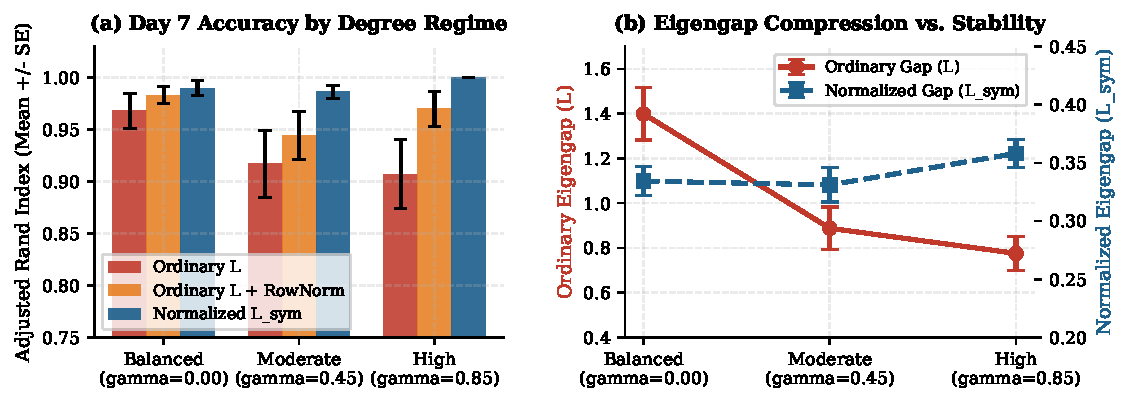
\includegraphics[width=0.92\textwidth]{figures/fig1_day7_ari_eigengap.pdf}
    \caption{Day 7 experimental results ($N=30, K=3, p_{\mathrm{in}}=0.65, p_{\mathrm{out}}=0.08$, 30 trials per condition). (a) Mean Adjusted Rand Index ($\pm$ standard error) for Ordinary $L$, Row-Normalized Ordinary $L$, and Symmetric Normalized $L_{\mathrm{sym}}$. (b) Compression of the ordinary eigengap $\lambda_4(L) - \lambda_3(L)$ under increasing degree heterogeneity contrasted with the invariance of $\lambda_4(L_{\mathrm{sym}}) - \lambda_3(L_{\mathrm{sym}})$.}
    \label{fig:day7}
\end{figure*}

\subsection{Day 8 Two-Way Regime Interaction \& Localization Results}
Stratifying the 90 Day 7 trials into terciles of realized mixing $\mu_{\mathrm{emp}} = m_{\mathrm{out}} / (m_{\mathrm{in}} + m_{\mathrm{out}})$ revealed that under Low Mixing ($\mu_{\mathrm{emp}} \le Q_{33}$, $\bar{\mu} \approx 0.18$), $\Delta\mathrm{ARI}$ under High degree imbalance was only $+0.0113$, whereas under High Mixing ($\mu_{\mathrm{emp}} > Q_{67}$, $\bar{\mu} \approx 0.25$), $\Delta\mathrm{ARI}$ jumped to $+0.1873$. Motivated by this observation, the Day 8 factorial experiment systematically varied $p_{\mathrm{out}} \in \{0.02, 0.06, 0.10, 0.15, 0.22\}$ across $\gamma \in \{0.00, 0.45, 0.85\}$ (450 graph instances).

Table~\ref{tab:day8_grid} and Figure~\ref{fig:day8_interaction} confirm Hypothesis H2:
\begin{itemize}\setlength{\itemsep}{1pt}\setlength{\parskip}{0pt}
    \item \textbf{High-Separation Regime ($p_{\mathrm{out}}=0.02, \bar{\mu}\approx 0.06$):} Both $L$ and $L_{\mathrm{sym}}$ achieve $\mathrm{ARI} = 1.0000$ across all 30 trials even under High degree heterogeneity ($\Delta\mathrm{ARI} = 0.0000$). Here, $\lambda_3(L)/d_{\min} \le 0.2523 \ll 1$, so the three community eigenvectors of $L$ lie far below the minimum-degree threshold.
    \item \textbf{Moderate-to-High Mixing Regimes ($p_{\mathrm{out}} \in [0.10, 0.22]$):} As inter-community bridges increase, $\lambda_3(L)$ rises toward $d_{\min}$. At $p_{\mathrm{out}}=0.15$ ($\bar{\mu}\approx 0.33$), $\Delta\mathrm{ARI}$ more than doubles across degree regimes from $+0.1280$ (Balanced) to $+0.2158$ (Moderate) and $+0.2702$ (High). At $p_{\mathrm{out}}=0.22$ ($\bar{\mu}\approx 0.42$), $\mathrm{ARI}_{\mathrm{ord}}$ collapses from $0.5672$ (Balanced) to $0.3335$ (High), while $\mathrm{ARI}_{\mathrm{norm}}$ remains at $0.8844$, producing $\Delta\mathrm{ARI} = +0.5509$ ($95\%$ CI $[+0.462, +0.640]$, winning $30/30$ trials).
\end{itemize}

\begin{table*}[!htbp]
\centering
\caption{Day 8 Two-Way Regime Interaction Study ($N=30, K=3, p_{\mathrm{in}}=0.65$, 30 trials per cell, 450 graphs total). Columns report empirical mixing $\bar{\mu}_{\mathrm{emp}}$, mean ARI, paired $\Delta\mathrm{ARI}$ with 95\% confidence intervals, two-sided Wilcoxon $p$-values, win/tie/loss counts ($W/T/L$), eigengaps, threshold ratio $\lambda_3(L)/d_{\min}$, Inverse Participation Ratio ($\mathrm{IPR}$), and squared norm on the minimum-degree vertex $\mathrm{MinDeg\ }E(L)$.}
\label{tab:day8_grid}
\resizebox{\textwidth}{!}{%
\begin{tabular}{llccccccccccccc}
\toprule
\textbf{$p_{\mathrm{out}}$} & \textbf{Regime} & \textbf{$\bar{\mu}_{\mathrm{emp}}$} & \textbf{Ord ARI} & \textbf{Norm ARI} & \textbf{$\Delta\mathrm{ARI}$} & \textbf{95\% CI} & \textbf{Wilcox $p$} & \textbf{$W/T/L$} & \textbf{Gap($L$)} & \textbf{Gap($L_{\mathrm{sym}}$)} & \textbf{$\lambda_3/d_{\min}$} & \textbf{$\mathrm{IPR}(L)$} & \textbf{$\mathrm{IPR}(L_{\mathrm{sym}})$} & \textbf{MinDeg $E(L)$} \\
\midrule
$0.02$ & Balanced & $0.0643$ & $1.0000$ & $1.0000$ & $+0.0000$ & $[+0.000, +0.000]$ & $1.00\times 10^{0}$  & $0/30/0$  & $2.1786$ & $0.5305$ & $0.1918$ & $0.0550$ & $0.0553$ & $0.1174$ \\
$0.02$ & Moderate & $0.0635$ & $1.0000$ & $1.0000$ & $+0.0000$ & $[+0.000, +0.000]$ & $1.00\times 10^{0}$  & $0/30/0$  & $1.7970$ & $0.5320$ & $0.2396$ & $0.0539$ & $0.0555$ & $0.1352$ \\
$0.02$ & High     & $0.0604$ & $1.0000$ & $1.0000$ & $+0.0000$ & $[+0.000, +0.000]$ & $1.00\times 10^{0}$  & $0/30/0$  & $1.7502$ & $0.5672$ & $0.2523$ & $0.0539$ & $0.0569$ & $0.1255$ \\
\midrule
$0.06$ & Balanced & $0.1616$ & $0.9830$ & $0.9966$ & $+0.0136$ & $[+0.000, +0.027]$ & $1.25\times 10^{-1}$ & $4/26/0$  & $1.7103$ & $0.4059$ & $0.4155$ & $0.0650$ & $0.0561$ & $0.1675$ \\
$0.06$ & Moderate & $0.1614$ & $0.9625$ & $1.0000$ & $+0.0375$ & $[-0.011, +0.087]$ & $2.50\times 10^{-1}$ & $3/27/0$  & $1.3003$ & $0.3939$ & $0.5084$ & $0.0804$ & $0.0565$ & $0.1989$ \\
$0.06$ & High     & $0.1662$ & $0.9650$ & $1.0000$ & $+0.0350$ & $[-0.001, +0.071]$ & $6.25\times 10^{-2}$ & $5/25/0$  & $1.2149$ & $0.4263$ & $0.5280$ & $0.0831$ & $0.0569$ & $0.2549$ \\
\midrule
$0.10$ & Balanced & $0.2427$ & $0.9357$ & $0.9830$ & $+0.0473$ & $[+0.013, +0.081]$ & $7.81\times 10^{-3}$ & $8/22/0$  & $1.3318$ & $0.2913$ & $0.5895$ & $0.0819$ & $0.0574$ & $0.2619$ \\
$0.10$ & Moderate & $0.2392$ & $0.9061$ & $0.9800$ & $+0.0740$ & $[+0.018, +0.130]$ & $3.91\times 10^{-3}$ & $9/21/0$  & $1.0569$ & $0.3083$ & $0.6813$ & $0.1105$ & $0.0579$ & $0.3209$ \\
$0.10$ & High     & $0.2485$ & $0.9240$ & $0.9800$ & $+0.0560$ & $[+0.006, +0.106]$ & $3.13\times 10^{-2}$ & $6/24/0$  & $0.8004$ & $0.3228$ & $0.7045$ & $0.1229$ & $0.0585$ & $0.3273$ \\
\midrule
$0.15$ & Balanced & $0.3289$ & $0.7951$ & $0.9232$ & $+0.1280$ & $[+0.061, +0.195]$ & $7.62\times 10^{-4}$ & $15/13/2$ & $1.0105$ & $0.1999$ & $0.7361$ & $0.1206$ & $0.0607$ & $0.3630$ \\
$0.15$ & Moderate & $0.3278$ & $0.7185$ & $0.9342$ & $+0.2158$ & $[+0.140, +0.291]$ & $8.78\times 10^{-5}$ & $20/10/0$ & $0.7516$ & $0.2050$ & $0.8438$ & $0.1827$ & $0.0604$ & $0.4908$ \\
$0.15$ & High     & $0.3245$ & $0.6867$ & $0.9568$ & $+0.2702$ & $[+0.159, +0.382]$ & $5.20\times 10^{-5}$ & $21/8/1$  & $0.6080$ & $0.2342$ & $0.8754$ & $0.2335$ & $0.0596$ & $0.6048$ \\
\midrule
$0.22$ & Balanced & $0.4169$ & $0.5672$ & $0.8465$ & $+0.2793$ & $[+0.193, +0.365]$ & $1.23\times 10^{-5}$ & $25/5/0$  & $0.8025$ & $0.1202$ & $0.8673$ & $0.1914$ & $0.0652$ & $0.4701$ \\
$0.22$ & Moderate & $0.4148$ & $0.4028$ & $0.8257$ & $+0.4229$ & $[+0.323, +0.522]$ & $3.78\times 10^{-6}$ & $28/2/0$  & $0.5473$ & $0.1189$ & $0.9705$ & $0.2486$ & $0.0640$ & $0.5847$ \\
$0.22$ & High     & $0.4166$ & $0.3335$ & $0.8844$ & $+0.5509$ & $[+0.462, +0.640]$ & $1.73\times 10^{-6}$ & $30/0/0$  & $0.4597$ & $0.1375$ & $0.9977$ & $0.3316$ & $0.0635$ & $0.7104$ \\
\bottomrule
\end{tabular}%
}
\end{table*}

\begin{figure*}[!htbp]
    \centering
    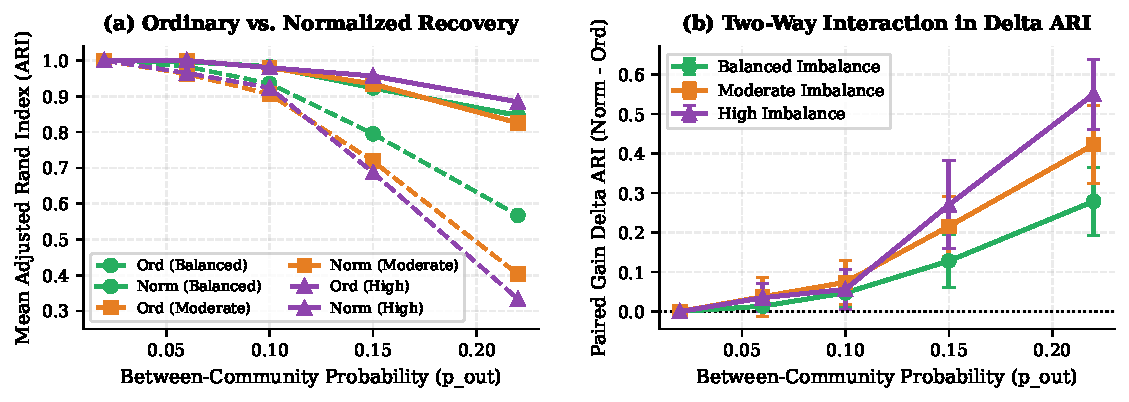
\includegraphics[width=0.92\textwidth]{figures/fig2_phase_interaction.pdf}
    \caption{Two-way interaction between degree heterogeneity ($\gamma$) and inter-community edge probability ($p_{\mathrm{out}}$) across 450 graphs. (a) Mean ARI trajectories for Ordinary $L$ (dashed) and Normalized $L_{\mathrm{sym}}$ (solid). (b) Paired accuracy gain $\Delta\mathrm{ARI}$ with 95\% confidence intervals, showing zero difference at $p_{\mathrm{out}}=0.02$ and super-additive divergence as $p_{\mathrm{out}} \to 0.22$.}
    \label{fig:day8_interaction}
\end{figure*}

\begin{figure*}[!htbp]
    \centering
    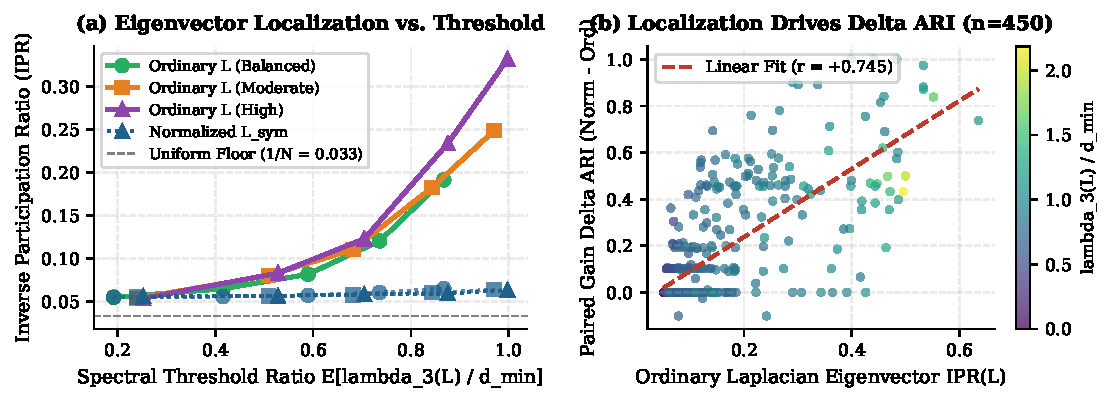
\includegraphics[width=0.92\textwidth]{figures/fig3_localization_mechanism.pdf}
    \caption{Mechanistic origin of ordinary spectral clustering failure. (a) Mean Inverse Participation Ratio ($\mathrm{IPR}$) plotted against the spectral threshold ratio $\mathbb{E}[\lambda_3(L)/d_{\min}]$, demonstrating sharp localization of $L$ eigenvectors as $\lambda_3(L) \to d_{\min}$ while $L_{\mathrm{sym}}$ remains delocalized ($\mathrm{IPR} \approx 0.06$). (b) Instance-level correlation ($r = +0.7453, n=450$) between $\mathrm{IPR}(L)$ and $\Delta\mathrm{ARI}$.}
    \label{fig:day8_localization}
\end{figure*}

\section{Statistical Analysis}
Because trial-level $\Delta\mathrm{ARI}_t$ values are bounded on $[-1, 2]$ and exhibit positive skewness when $\mathrm{ARI}_{\mathrm{norm}, t}$ saturates at $1.0000$ (resulting in many exact ties $\Delta\mathrm{ARI}_t = 0$ alongside large positive spikes when $L$ suffers eigenvector localization), relying solely on a parametric paired Student's $t$-test could be sensitive to departures from normality. We therefore report both two-sided paired $t$-tests with 95\% confidence intervals ($\mathrm{df}=29$) and non-parametric two-sided Wilcoxon signed-rank tests alongside exact win/tie/loss counts ($W/T/L$).

In Day 7 (Table~\ref{tab:day7_main}), both tests reach identical conclusions: under Balanced degrees ($\gamma=0.00$), $\Delta\mathrm{ARI} = +0.0220$ is not statistically distinguishable from zero ($t = 1.4012, p = 0.1718$; Wilcoxon $W = 0.0, p = 0.2500$; $3/27/0$). Under Moderate imbalance ($\gamma=0.45$), $\Delta\mathrm{ARI} = +0.0694$ is statistically significant ($t = 2.2719, p = 0.0307$; Wilcoxon $p = 0.0313$; $6/24/0$), and under High imbalance ($\gamma=0.85$), $\Delta\mathrm{ARI} = +0.0927$ is highly significant ($t = 2.8040, p = 0.0089$; Wilcoxon $p = 0.0156$; $7/23/0$). Across all 90 Day 7 trials, normalized spectral clustering never underperforms ordinary spectral clustering on a single graph instance ($0$ losses).

Across all $450$ instances in the Day 8 factorial grid, Pearson correlations confirm the theoretical perturbation links: $\mathrm{Gap}(L)$ correlates with $\mathrm{ARI}_{\mathrm{ord}}$ at $r = +0.5398$, $\mathrm{Gap}(L_{\mathrm{sym}})$ correlates with $\mathrm{ARI}_{\mathrm{norm}}$ at $r = +0.5087$, the threshold ratio $\lambda_3(L)/d_{\min}$ correlates with $\mathrm{ARI}_{\mathrm{ord}}$ at $r = -0.6557$, and eigenvector localization $\mathrm{IPR}(L)$ correlates with $\mathrm{ARI}_{\mathrm{ord}}$ at $r = -0.7494$ and with $\Delta\mathrm{ARI}$ at $r = +0.7453$ (Figure~\ref{fig:day8_localization}b).

\section{Discussion}
Our empirical findings reconcile two seemingly conflicting intuitions in spectral clustering. On one hand, degree heterogeneity alone does not automatically break the ordinary Laplacian $L$: when communities are weakly coupled ($p_{\mathrm{out}}=0.02$), the community cut eigenvalues $\lambda_2(L), \lambda_3(L)$ remain near zero ($\lambda_3(L)/d_{\min} \approx 0.25$), well separated from the minimum vertex degree $d_{\min}$. In this regime, the bottom $k$ eigenvectors of $L$ remain approximately piecewise-constant community indicators ($\mathrm{IPR}(L) = 0.0539$), and ordinary spectral clustering achieves $100\%$ recovery.

On the other hand, as inter-community edge density rises ($p_{\mathrm{out}} \ge 0.08$), $\lambda_2(L)$ and $\lambda_3(L)$ scale upward with the cut size while high degree heterogeneity pushes $d_{\min}$ downward. Once $\lambda_3(L)/d_{\min}$ approaches unity (reaching $0.9977$ at $p_{\mathrm{out}}=0.22, \gamma=0.85$), the $k$-th eigenvalue enters the continuous degree spectrum $[d_{\min}, d_{\max}]$ described by von Luxburg et al.\ \cite{vonluxburg2008consistency}. By the Courant--Fischer theorem, a unit vector concentrated on the minimum-degree vertex $i_{\min}$ achieves Rayleigh quotient $e_{i_{\min}}^T L e_{i_{\min}} = d_{\min}$, making it energetically cheaper for $L$ to place a localized spike on $i_{\min}$ inside the bottom-$k$ eigenspace than to represent the third community cut. Indeed, Table~\ref{tab:day8_grid} shows that at $(p_{\mathrm{out}}=0.22, \gamma=0.85)$, the single lowest-degree vertex absorbs $71.04\%$ of an entire eigenvector's squared norm ($\mathrm{MinDeg\ }E(L) = 0.7104$).

\section{Failure-Case Analysis}
Inspection of individual failure instances reveals two distinct structural failure modes:
\begin{enumerate}\setlength{\itemsep}{1pt}\setlength{\parskip}{0pt}
    \item \textbf{Peripheral Singleton Splitting in Ordinary Clustering ($L$):} In Day 7 under Moderate imbalance ($\gamma=0.45$), Ordinary clustering fails ($\mathrm{ARI}_{\mathrm{ord}} < 0.5$) on 2 of 30 trials while Normalized clustering fails on 0 (0 joint failures). In these failed trials, $u_3(L)$ localizes onto a degree-2 peripheral vertex, causing $k$-means to allocate an entire cluster to 1--2 peripheral nodes and merge two planted 10-node communities into a 20-node cluster ($\mathrm{ARI} \approx 0.44$).
    \item \textbf{Disconnected and Pendant-Vertex Instability in Standard Normalized Clustering ($L_{\mathrm{sym}}$):} To determine when $L_{\mathrm{sym}}$ loses its advantage, Table~\ref{tab:sparse} and Figure~\ref{fig:sparse} evaluate sparse high-heterogeneity regimes. When density drops to $(p_{\mathrm{in}}=0.32, p_{\mathrm{out}}=0.03, \gamma=1.00)$, the mean minimum degree falls to $\bar{d}_{\min} = 0.17$ and the mean number of connected components rises to $3.07$. Because every isolated vertex or disconnected pair creates an exact zero eigenvalue in $L_{\mathrm{sym}}$, the bottom $k=3$ eigenvectors are consumed by trivial component indicators, causing standard $L_{\mathrm{sym}}$ accuracy to collapse to $\mathrm{ARI} = 0.2134$ (nearly matching Ordinary $L$ at $0.1632$). Adding degree regularization $D_\tau = D + \tau I$ ($\tau = 0.25\bar{d}$) suppresses small-degree variance and restores recovery to $\mathrm{ARI} = 0.7357$.
\end{enumerate}

\begin{table}[!htbp]
\centering
\caption{Sparse Peripheral Vulnerability Study (30 trials per regime). Standard $L_{\mathrm{sym}}$ breaks down when $d_{\min} \to 0$ and components $>1$, whereas regularized $L_\tau$ ($\tau=0.25\bar{d}$) maintains recovery.}
\label{tab:sparse}
\resizebox{\linewidth}{!}{%
\begin{tabular}{lcccccc}
\toprule
\textbf{Sparse Regime} & \textbf{$\bar{d}_{\min}$} & \textbf{Comp} & \textbf{Ord} & \textbf{Ord+RN} & \textbf{Norm} & \textbf{Reg $L_\tau$} \\
\midrule
Dense ($0.65, 0.08, \gamma=0.85$)   & $2.90$ & $1.00$ & $0.9053$ & $0.9594$ & $0.9932$ & $0.9932$ \\
Mod.\ Sparse ($0.45, 0.05, 0.85$)   & $0.97$ & $1.20$ & $0.5894$ & $0.6966$ & $0.8448$ & $0.9200$ \\
Ext.\ Sparse ($0.32, 0.03, 1.00$)   & $0.17$ & $3.07$ & $0.1632$ & $0.1944$ & $0.2134$ & $0.7357$ \\
\bottomrule
\end{tabular}%
}
\end{table}

\begin{figure}[!htbp]
    \centering
    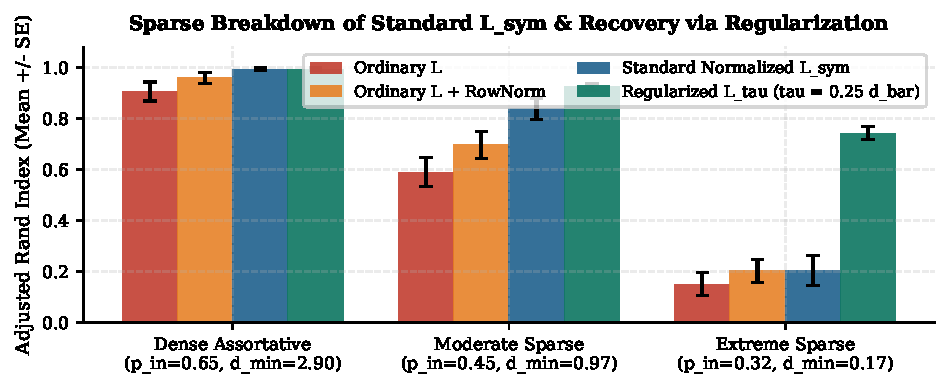
\includegraphics[width=\linewidth]{figures/fig4_sparse_regularization.pdf}
    \caption{Breakdown of standard $L_{\mathrm{sym}}$ in the sparse hub-periphery regime as $d_{\min} \to 0$ and recovery via degree-regularized $L_\tau$ ($\tau = 0.25\bar{d}$).}
    \label{fig:sparse}
\end{figure}

\section{Limitations}
Several scope boundaries qualify our conclusions:
\begin{enumerate}\setlength{\itemsep}{1pt}\setlength{\parskip}{0pt}
    \item \textbf{Finite Network Scale ($N=30$):} Our experiments focus on $N=30, K=3$ graphs to maintain continuity with the project's baseline benchmarks and permit exact dense eigendecompositions across 630 total graph instances. At larger scales ($N \ge 10^3$), power-law degree tails can span several orders of magnitude, sharpening the localization transition.
    \item \textbf{Equal Planted Community Sizes ($n_c=10$):} We deliberately held community sizes and expected volumes equal across all three communities to isolate vertex-level degree dispersion from community-volume imbalance.
    \item \textbf{Known Cluster Count ($k=3$):} All pipelines were supplied the true number of communities $k=3$ rather than estimating $k$ automatically from eigengap heuristics.
\end{enumerate}

\section{Conclusion}
By decoupling within-community degree heterogeneity from inter-community mixing through a Separation-Calibrated DC-SBM, this study demonstrates that the advantage of symmetric normalized spectral clustering ($L_{\mathrm{sym}}$) over ordinary spectral clustering ($L$) is governed by a fundamental interaction between degree dispersion and community separation. When $\lambda_k(L) \ll d_{\min}$, both operators recover planted communities accurately. When increasing degree heterogeneity or inter-community mixing drives $\lambda_k(L)/d_{\min} \to 1$, the ordinary eigengap $\lambda_{k+1}(L) - \lambda_k(L)$ collapses and the nontrivial eigenvectors of $L$ localize sharply onto minimum-degree peripheral vertices ($r = -0.7494$ with $\mathrm{ARI}_{\mathrm{ord}}$), causing severe clustering failures that spherical row normalization alone cannot fully repair. Conversely, in ultra-sparse hub-periphery networks where $d_{\min} \to 0$, standard $L_{\mathrm{sym}}$ itself degrades due to disconnected and pendant vertices, requiring degree regularization ($L_\tau$) for reliable community detection.

\section{Future Work}
Promising extensions of this work include: (1) evaluating the random-walk Laplacian $L_{\mathrm{rw}} = D^{-1}L$ and entrywise eigenvector-ratio embeddings (SCORE) under joint degree and community-size heterogeneity; (2) deriving data-driven selection rules for the regularization parameter $\tau$ in $L_\tau$ based on empirical degree quantiles; and (3) scaling the benchmark to sparse Lanczos solvers (\texttt{scipy.sparse.linalg.eigsh}) on real-world citation and social networks.

\bibliographystyle{plain}
\bibliography{references}

\end{document}
